% !TEX TS-program = lualatex
% !TEX encoding = UTF-8 Unicode

\documentclass[professionalfonts]{beamer}
\usepackage{iftex,ifxetex}
\ifPDFTeX
  \usepackage[utf8]{inputenc}
  \usepackage[T1]{fontenc}
  \usepackage{lmodern}
\else
  \ifluatex
    \usepackage{unicode-math} 
    \defaultfontfeatures{Ligatures=TeX}
    % \setmathfont{Latin Modern Math}
    \setsansfont{CMU Sans Serif}
    % \setsansfont{Linux Biolinum O}
  \fi
\fi

\mode<presentation>
{
  \usetheme{Madrid} % or try Darmstadt, Madrid, Warsaw, ...
  % or ...
  \setbeamertemplate{bibliography item}{}
  \setbeamercovered{transparent}
  % or whatever (possibly just delete it)
}

\usepackage{fontspec}
\usepackage[english]{babel}
% or whatever
\usepackage{csquotes}
\usepackage[backend=biber,
        style=unified,
        maxcitenames=3,
        maxbibnames=99,
        natbib,
        url=false]{biblatex}
% \addbibresource{Dissertation.bib}
\setmainfont{Libertinus Sans} % Main font
% \setsansfont{libertinus sansserif} % Sans serif font
% \setmonofont{CMU Typewriter Text}
\renewcommand{\ttdefault}{cmtt}

% \usepackage[colorlinks,allcolors={black},urlcolor={blue}]{hyperref} %allows for hyperlinks and pdf bookmarks 
\usepackage{graphicx}	%Inserting graphics, pictures, images 		
\usepackage{multicol} %Multicolumn text
\usepackage{multirow} %Useful for combining cells in tablesbrew 
% \usepackage{booktabs} %Enhanced tables
% \usepackage{underscore} %Allows for underscores in text mode
% \usepackage[colorlinks,allcolors={black},urlcolor={blue}]{hyperref} %allows for hyperlinks and pdf bookmarks
\usepackage{url} %allows for urls
\def\UrlBreaks{\do\/\do-} %allows for urls to be broken up
% \usepackage[normalem]{ulem} %strike out text. Handy for syntax
% \usepackage{tcolorbox}
% \usepackage{datetime2}
\usepackage{caption}
\usepackage{subcaption}
\usepackage{langsci-gb4e} % Language Science Press' modification of gb4e
\usepackage{tikz} % Drawing Hasse diagrams
\usetikzlibrary{decorations.pathreplacing,positioning}
\usepackage{leipzig} %	Offers support for Leipzig Glossing Rules
% \usepackage{animate} % For creating animations in PDF slides
\usepackage{annotate-equations}

% Okabe–Ito color palette
\definecolor{voicing}{HTML}{56B4E9}    % Sky blue
\definecolor{closure}{HTML}{F0E442}    % Yellow
\definecolor{release}{HTML}{D55E00}    % Vermillion
\definecolor{aspiration}{HTML}{009E73} % Bluish green

% Hyperlink settings
\hypersetup{
    colorlinks,
    urlcolor=blue,        % Color for URLs
    linkcolor=white        % Color for internal links
}

\title[LING 450/550] % (optional, use only with long paper titles)
{Introduction to Linguistic Phonetics}

\subtitle{Consonant Acoustics}

\author[Brinkerhoff] % (optional, use only with lots of authors)
{Mykel Loren Brinkerhoff}
% - Give the names in the same order as the appear in the paper.
% - Use the \inst{?} command only if the authors have different
%   affiliation.

\institute[UW] % (optional, but mostly needed)
{University of Washington}
% - Use the \inst command only if there are several affiliations.

\date[2025-10-21] % (optional, should be abbreviation of conference name)
{October 21, 2025}

% If you have a file called "university-logo-filename.xxx", where xxx
% is a graphic format that can be processed by latex or pdflatex,
% resp., then you can add a logo as follows:

% \pgfdeclareimage[height=0.5cm]{university-logo}{university-logo-filename}
% \logo{\pgfuseimage{university-logo}}



% Delete this, if you do not want the table of contents to pop up at
% the beginning of each subsection:
% \AtBeginSubsection[]
% {
%   \begin{frame}<beamer>{Outline}
%     \tableofcontents[currentsection,currentsubsection]
%   \end{frame}
% }


% If you wish to uncover everything in a step-wise fashion, uncomment
% the following command: 

%\beamerdefaultoverlayspecification{<+->}


\begin{document}

\begin{frame}
    \titlepage
\end{frame}

%-----------------------------------------------------------
\section{Introduction}
%-----------------------------------------------------------

% \begin{frame}{Which medieval cat are you?}
    
%     \begin{center}
%         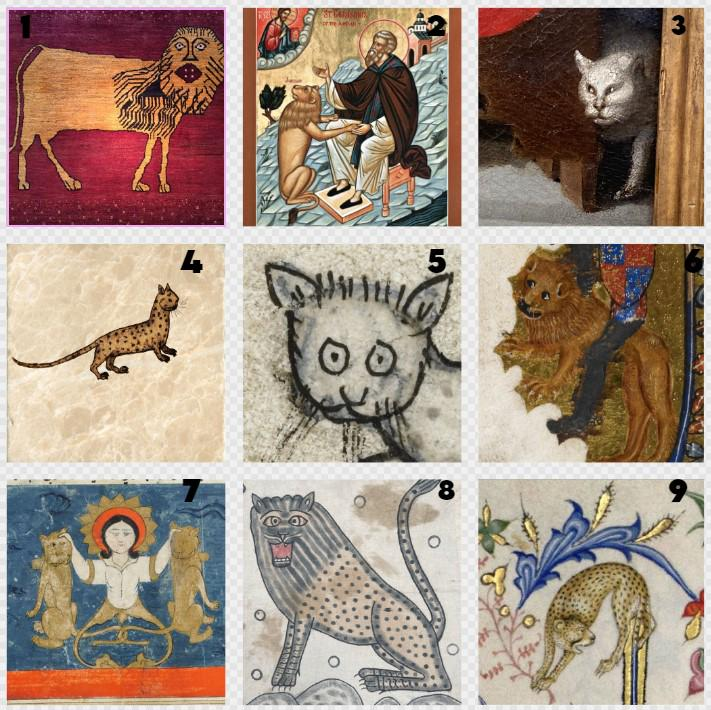
\includegraphics[width = .5\linewidth]{figs/MedievalCatIcebreaker.jpeg}
%         \url{https://pollev.com/mykellorenbrinkerhoff821} or text/SMS mykellorenbrinkerhoff821 to 22333
%     \end{center}
% \end{frame}

\begin{frame}{Recap and Reflection}
    \begin{block}{Reflection}
        \begin{itemize}
            \item Spend $\thicksim$3 minutes reviewing your notes from last lecture, homeworks, exit tickets, etc.
            \item Look for questions you have or clarifications you would like. 
        \end{itemize}
    \end{block}
\end{frame}

\begin{frame}{Voice Onset Time (VOT)}
\centering
    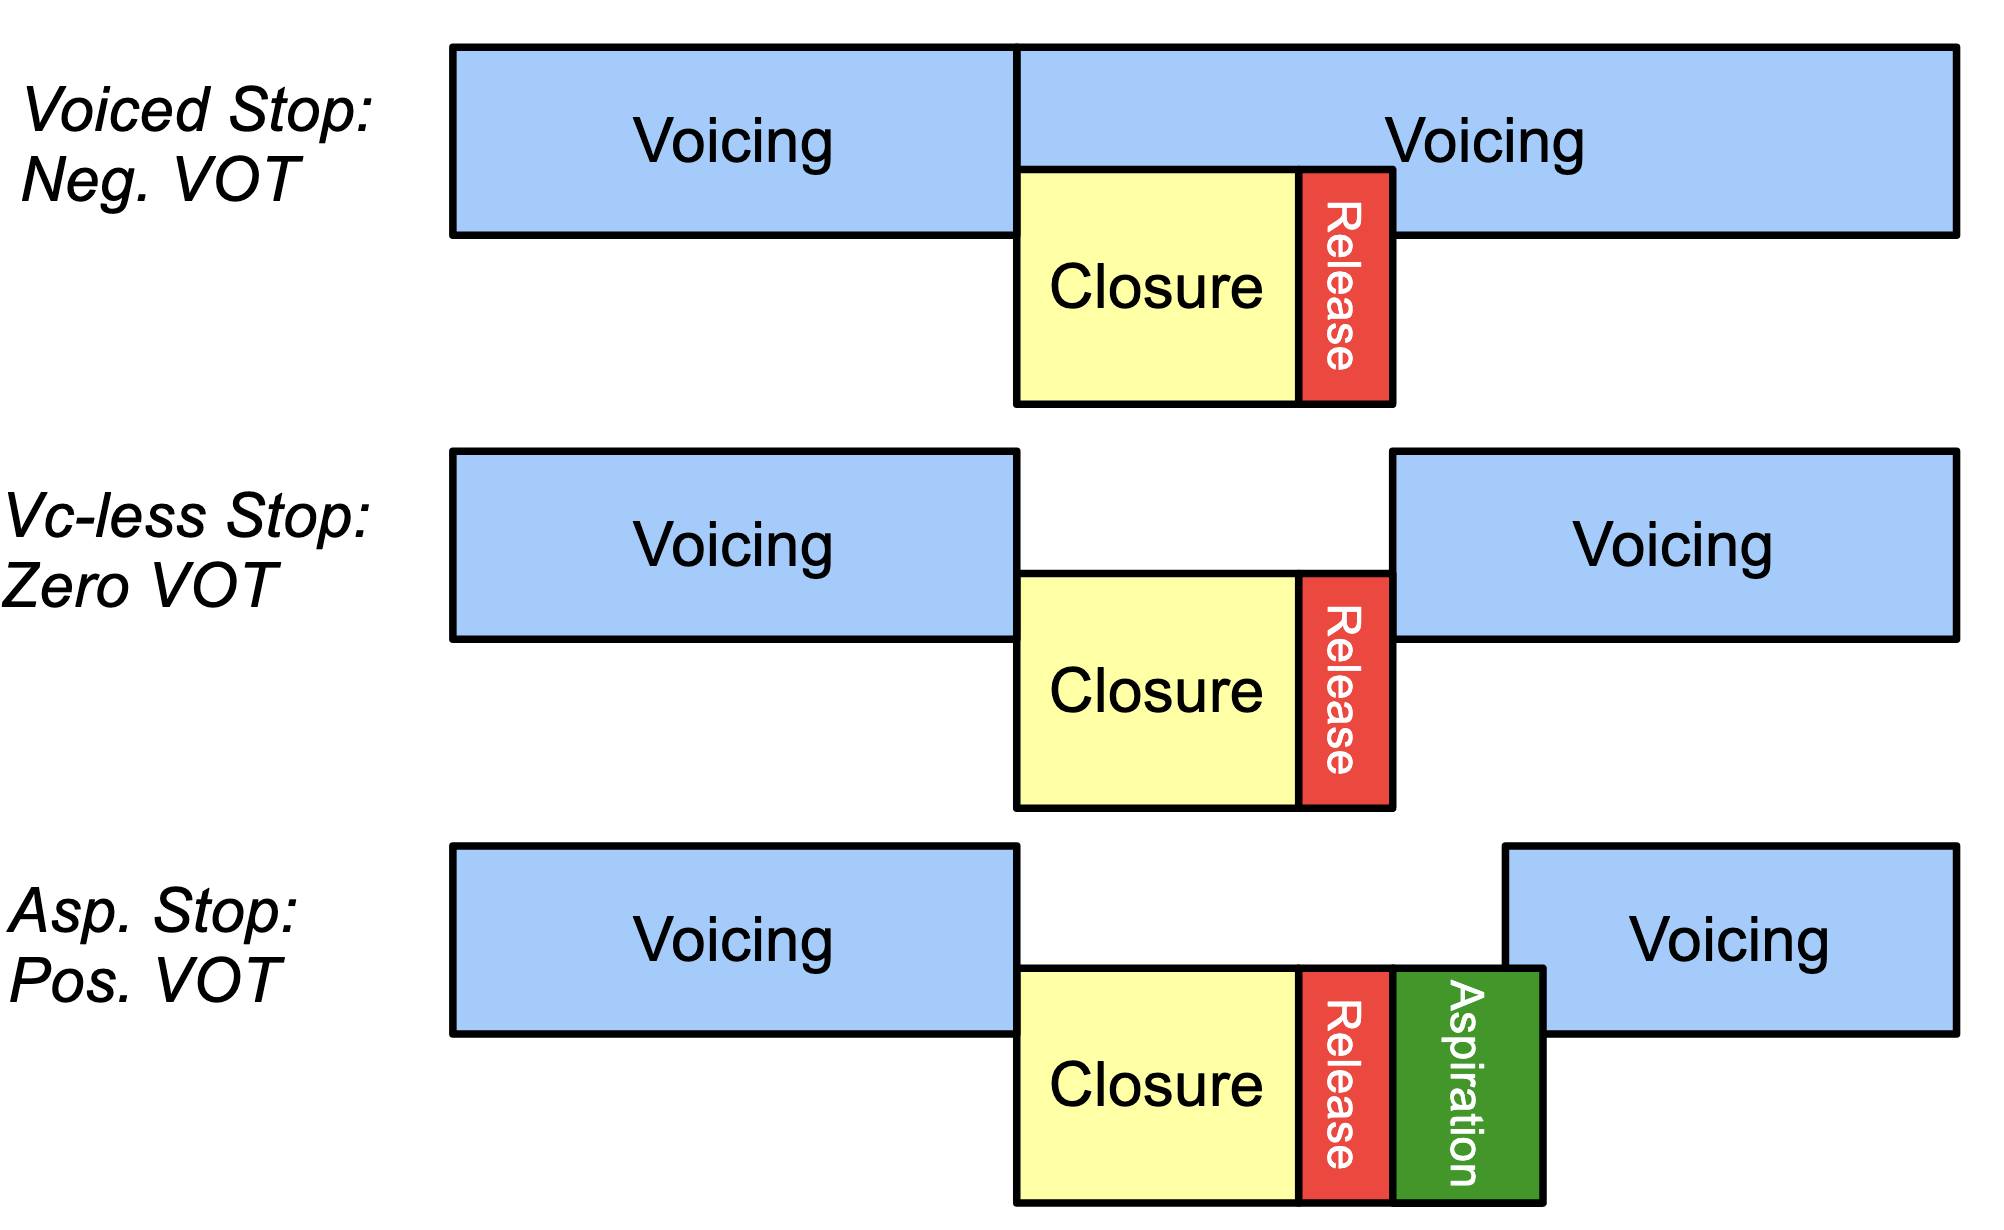
\includegraphics[width = \textwidth]{figs/VOT.png}
\end{frame}
% %-----------------------------------------------------------
% \section*{Break}
% %-----------------------------------------------------------

% \begin{frame}{Break Time!}
%     \begin{center}
%         \Huge 10 minute break \\ (stretch, grab a drink, etc.)
%     \end{center}
% \end{frame}



%-----------------------------------------------------------
\section*{To Do:}
%-----------------------------------------------------------
\begin{frame}{To Do:}
    \begin{itemize}
        \item Complete the exit ticket for today on Canvas by 12:30pm.
        \item Submit your discussion posts on the readings
        \item Bring your computers for next time, we'll be playing with Praat and sound waves!!!
    \end{itemize}
\end{frame}

% \subsection<presentation>*{References}
% %-----------------------------------------------------------
% \begin{frame}[t,allowframebreaks]
%   \frametitle<presentation>{References}
%     \printbibliography
% \end{frame}

\end{document}